% Graphic for TeX using PGF
% Title: /home/tom/Documents/BeginningFunctionalAnalysis/figures/1_1_2_b.dia
% Creator: Dia v0.97.3
% CreationDate: Fri Feb 16 22:11:45 2018
% For: tom
% \usepackage{tikz}
% The following commands are not supported in PSTricks at present
% We define them conditionally, so when they are implemented,
% this pgf file will use them.
\ifx\du\undefined
  \newlength{\du}
\fi
\setlength{\du}{15\unitlength}
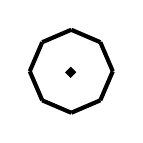
\begin{tikzpicture}
\pgftransformxscale{1.000000}
\pgftransformyscale{-1.000000}
\definecolor{dialinecolor}{rgb}{0.000000, 0.000000, 0.000000}
\pgfsetstrokecolor{dialinecolor}
\definecolor{dialinecolor}{rgb}{1.000000, 1.000000, 1.000000}
\pgfsetfillcolor{dialinecolor}
\pgfsetlinewidth{0.150000\du}
\pgfsetdash{}{0pt}
\pgfsetdash{}{0pt}
\pgfsetbuttcap
\pgfsetmiterjoin
\pgfsetlinewidth{0.150000\du}
\pgfsetbuttcap
\pgfsetmiterjoin
\pgfsetdash{}{0pt}
\definecolor{dialinecolor}{rgb}{1.000000, 1.000000, 1.000000}
\pgfsetfillcolor{dialinecolor}
\pgfpathellipse{\pgfpoint{18.986047\du}{17.025649\du}}{\pgfpoint{0.025394\du}{0\du}}{\pgfpoint{0\du}{0.025394\du}}
\pgfusepath{fill}
\definecolor{dialinecolor}{rgb}{0.000000, 0.000000, 0.000000}
\pgfsetstrokecolor{dialinecolor}
\pgfpathellipse{\pgfpoint{18.986047\du}{17.025649\du}}{\pgfpoint{0.025394\du}{0\du}}{\pgfpoint{0\du}{0.025394\du}}
\pgfusepath{stroke}
\pgfsetbuttcap
\pgfsetmiterjoin
\pgfsetdash{}{0pt}
\definecolor{dialinecolor}{rgb}{0.000000, 0.000000, 0.000000}
\pgfsetstrokecolor{dialinecolor}
\pgfpathellipse{\pgfpoint{18.986047\du}{17.025649\du}}{\pgfpoint{0.025394\du}{0\du}}{\pgfpoint{0\du}{0.025394\du}}
\pgfusepath{stroke}
\pgfsetlinewidth{0.100000\du}
\pgfsetdash{}{0pt}
\pgfsetdash{}{0pt}
\pgfsetbuttcap
{
\definecolor{dialinecolor}{rgb}{0.000000, 0.000000, 0.000000}
\pgfsetfillcolor{dialinecolor}
% was here!!!
\definecolor{dialinecolor}{rgb}{0.000000, 0.000000, 0.000000}
\pgfsetstrokecolor{dialinecolor}
\draw (19.700000\du,16.300000\du)--(20.000000\du,17.000000\du);
}
\pgfsetlinewidth{0.100000\du}
\pgfsetdash{}{0pt}
\pgfsetdash{}{0pt}
\pgfsetbuttcap
{
\definecolor{dialinecolor}{rgb}{0.000000, 0.000000, 0.000000}
\pgfsetfillcolor{dialinecolor}
% was here!!!
\definecolor{dialinecolor}{rgb}{0.000000, 0.000000, 0.000000}
\pgfsetstrokecolor{dialinecolor}
\draw (19.000000\du,16.000000\du)--(19.700000\du,16.300000\du);
}
\pgfsetlinewidth{0.100000\du}
\pgfsetdash{}{0pt}
\pgfsetdash{}{0pt}
\pgfsetbuttcap
{
\definecolor{dialinecolor}{rgb}{0.000000, 0.000000, 0.000000}
\pgfsetfillcolor{dialinecolor}
% was here!!!
\definecolor{dialinecolor}{rgb}{0.000000, 0.000000, 0.000000}
\pgfsetstrokecolor{dialinecolor}
\draw (19.700000\du,17.700000\du)--(20.000000\du,17.000000\du);
}
\pgfsetlinewidth{0.100000\du}
\pgfsetdash{}{0pt}
\pgfsetdash{}{0pt}
\pgfsetbuttcap
{
\definecolor{dialinecolor}{rgb}{0.000000, 0.000000, 0.000000}
\pgfsetfillcolor{dialinecolor}
% was here!!!
\definecolor{dialinecolor}{rgb}{0.000000, 0.000000, 0.000000}
\pgfsetstrokecolor{dialinecolor}
\draw (19.000000\du,18.000000\du)--(19.700000\du,17.700000\du);
}
\pgfsetlinewidth{0.100000\du}
\pgfsetdash{}{0pt}
\pgfsetdash{}{0pt}
\pgfsetbuttcap
{
\definecolor{dialinecolor}{rgb}{0.000000, 0.000000, 0.000000}
\pgfsetfillcolor{dialinecolor}
% was here!!!
\definecolor{dialinecolor}{rgb}{0.000000, 0.000000, 0.000000}
\pgfsetstrokecolor{dialinecolor}
\draw (18.300000\du,17.700000\du)--(19.000000\du,18.000000\du);
}
\pgfsetlinewidth{0.100000\du}
\pgfsetdash{}{0pt}
\pgfsetdash{}{0pt}
\pgfsetbuttcap
{
\definecolor{dialinecolor}{rgb}{0.000000, 0.000000, 0.000000}
\pgfsetfillcolor{dialinecolor}
% was here!!!
\definecolor{dialinecolor}{rgb}{0.000000, 0.000000, 0.000000}
\pgfsetstrokecolor{dialinecolor}
\draw (18.000000\du,17.000000\du)--(18.300000\du,17.700000\du);
}
\pgfsetlinewidth{0.100000\du}
\pgfsetdash{}{0pt}
\pgfsetdash{}{0pt}
\pgfsetbuttcap
{
\definecolor{dialinecolor}{rgb}{0.000000, 0.000000, 0.000000}
\pgfsetfillcolor{dialinecolor}
% was here!!!
\definecolor{dialinecolor}{rgb}{0.000000, 0.000000, 0.000000}
\pgfsetstrokecolor{dialinecolor}
\draw (18.300000\du,16.300000\du)--(18.000000\du,17.000000\du);
}
\pgfsetlinewidth{0.100000\du}
\pgfsetdash{}{0pt}
\pgfsetdash{}{0pt}
\pgfsetbuttcap
{
\definecolor{dialinecolor}{rgb}{0.000000, 0.000000, 0.000000}
\pgfsetfillcolor{dialinecolor}
% was here!!!
\definecolor{dialinecolor}{rgb}{0.000000, 0.000000, 0.000000}
\pgfsetstrokecolor{dialinecolor}
\draw (19.000000\du,16.000000\du)--(18.300000\du,16.300000\du);
}
\end{tikzpicture}
